% 先端芸術音楽創作学会会報テンプレート ver.200908
% By Daichi Ando
% based on ICMC2005

\documentclass{jsarticle}
\renewcommand{\baselinestretch}{0.9}
\usepackage{jssa,amsmath}
\usepackage{mediabb}
\usepackage{graphicx}
\usepackage{plext}

\def\boutenchar{・}

% Title.
% ------
% LaTeX環境によっては,maketitleでエラーが出ることもあるが,強行して良い

\title{日本語タイトル \\ 
―日本語タイトル2行目― \\
English Tile: \\
English Title Second Line\\
}

% Paper Category 論文,報告,連載,書評……など
\category{カテゴリー}

% Single address
% To use with only one author or several with the same address
% ---------------
\oneauthor
  {著者氏名 \\ Author's Name} 
  {所属 \\
  School Department}

% Two addresses
% --------------
%\twoauthors
%  {First author} {School \\ Department}
%  {Second author} {Company \\ Address}

% Three addresses
% --------------
%\threeauthors
%  {First author} {School \\ Department}
%  {Second author} {Company \\ Address}
%  {Third author} {Company \\ Address}

\begin{document}
%
%%% --ページ数等の指定
\makeatletter 
\def\ps@myheadings{% 
\let\ps@jpl@in\ps@plain% 
\def\@evenhead{\reset@font\hfil\leftmark\hfil}% 
\def\@oddhead{\reset@font\hfil\rightmark\hfil}% 
\let\@mkboth\@gobbletwo% 
\let\sectionmark\@gobble% 
\let\subsectionmark\@gobble% 
% 
\def\@oddfoot{\reset@font\hfil-- \thepage --\hfil}% 
\let\@evenfoot\@oddfoot 
} 
\makeatother 

%%% 
%%% 開始ページ数を設定する 
%投稿の段階では無視

\setcounter{page}{ 9 } 
\pagestyle{myheadings} 

%%% 
%%% 論文のVol., No., pp.を設定する 
% 投稿の段階では無視

\markright{\footnotesize \gt 先端芸術音楽創作学会 会報 Vol.1 No.1 pp.9--16 }

%%% 
%%% \maketitleの直後の行に \thispagestyle{myheadings} を挿入する。 

\maketitle
\thispagestyle{myheadings}

%
\begin{abstract}

日本語概要.この部分には日本語概要である.日本語概要.日本語概要.日本語
 概要.日本語概要.日本語概要.日本語概要.日本語概要.日本語概要.日本
 語概要.日本語概要.日本語概要.日本語概要.日本語概要.日本語概要.日
 本語概要.日本語概要.日本語概要.日本語概要.日本語概要.\\


English Abstract. This section is English Abstract. English
 Abstract. English Abstract. English Abstract. English Abstract. English
 Abstract. English Abstract. English Abstract. English Abstract. English
 Abstract. 


\end{abstract}
%
\section{はじめに}

基本的に全ての記法は通常のLaTeXのものを用いる.

見出しは以下のとおりである.

\subsection{subsection}

ここが \verb|\subsection{}|.

\subsubsection{subsubsection}

ここが \verb|\subsubsection{}|.


\section{図の挿入}

以下のようにして図を挿入する.

figure環境で[h]オプションをつけることにより``可能ならば''図が指示した場
所に入れることができる.

\begin{figure}[h]
\centerline{
	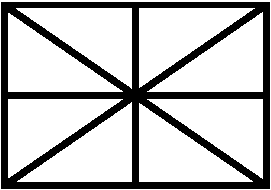
\includegraphics[mediaboxonly,width=\columnwidth]{figure.pdf}
}
\caption{日本語キャプション}
\label{fig:figure}
\end{figure}

\section{脚注}

以下のようにして脚注を挿入する\footnote{これが脚注部分}.

\section{参考文献}

以下のようにして参考文献を引く\cite{Author1:08}.

このようにも引ける\cite{Author1:08,Author2:09}

\section{文字数カウント用}

日本語日本語日本語日本語日本語日本語日本語日本語日本語日本語日本語日本語
日本語日本語日本語日本語日本語日本語日本語日本語日本語日本語日本語日本語
日本語日本語日本語日本語日本語日本語日本語日本語日本語日本語日本語日本語
日本語日本語日本語日本語日本語日本語日本語日本語日本語日本語日本語日本語
日本語日本語日本語日本語日本語日本語日本語日本語日本語日本語日本語日本語
日本語日本語日本語日本語日本語日本語日本語日本語日本語日本語日本語日本語
日本語日本語日本語日本語日本語日本語日本語日本語日本語日本語日本語日本語
日本語日本語日本語日本語日本語日本語日本語日本語日本語日本語日本語日本語
日本語日本語日本語日本語日本語日本語日本語日本語日本語日本語日本語日本語
日本語日本語日本語日本語日本語日本語日本語日本語日本語日本語日本語日本語
日本語日本語日本語日本語日本語日本語日本語日本語日本語日本語日本語日本語
日本語日本語日本語日本語日本語日本語日本語日本語日本語日本語日本語日本語
日本語日本語日本語日本語日本語日本語日本語日本語

日本語日本語日本語日本語日本語日本語日本語日本語日本語日本語日本語日本語
日本語日本語日本語日本語日本語日本語日本語日本語日本語日本語日本語日本語
日本語日本語日本語日本語日本語日本語日本語日本語日本語日本語日本語日本語
日本語日本語日本語日本語日本語日本語日本語日本語日本語日本語日本語日本語
日本語日本語日本語日本語日本語日本語日本語日本語日本語日本語日本語日本語
日本語日本語日本語日本語日本語日本語日本語日本語日本語日本語日本語日本語
日本語日本語日本語日本語日本語日本語日本語日本語日本語日本語日本語日本語
日本語日本語日本語日本語日本語日本語日本語日本語日本語日本語日本語日本語
日本語日本語日本語日本語日本語日本語日本語日本語日本語日本語日本語日本語
日本語日本語日本語日本語日本語日本語日本語日本語日本語日本語日本語日本語
日本語日本語日本語日本語日本語日本語日本語日本語日本語日本語日本語日本語
日本語日本語日本語日本語日本語日本語日本語日本語日本語日本語日本語日本語
日本語日本語日本語日本語日本語日本語日本語日本語日本語日本語日本語日本語
日本語日本語日本語日本語日本語日本語

日本語日本語日本語日本語日本語日本語日本語日本語日本語日本語日本語日本語
日本語日本語日本語日本語日本語日本語日本語日本語日本語日本語日本語日本語
日本語日本語日本語日本語日本語日本語日本語日本語日本語日本語日本語日本語
日本語日本語日本語日本語日本語日本語日本語日本語日本語日本語日本語日本語
日本語日本語日本語日本語日本語日本語日本語日本語日本語日本語日本語日本語
日本語日本語日本語日本語日本語日本語日本語日本語日本語日本語日本語日本語
日本語日本語日本語日本語日本語日本語日本語日本語日本語日本語日本語日本語
日本語日本語日本語日本語日本語日本語日本語日本語日本語日本語日本語日本語
日本語日本語日本語日本語日本語日本語日本語日本語日本語日本語日本語日本語
日本語日本語日本語日本語日本語日本語日本語日本語日本語日本語日本語日本語
日本語日本語日本語日本語日本語日本語日本語日本語日本語日本語日本語日本語
日本語日本語日本語日本語日本語日本語日本語日本語日本語日本語日本語日本語
日本語日本語日本語日本語日本語日本語日本語日本語

日本語日本語日本語日本語日本語日本語日本語日本語日本語日本語日本語日本語
日本語日本語日本語日本語日本語日本語日本語日本語日本語日本語日本語日本語
日本語日本語日本語日本語日本語日本語日本語日本語日本語日本語日本語日本語
日本語日本語日本語日本語日本語日本語日本語日本語日本語日本語日本語日本語
日本語日本語日本語日本語日本語日本語日本語日本語日本語日本語日本語日本語
日本語日本語日本語日本語日本語日本語日本語日本語日本語日本語日本語日本語
日本語日本語日本語日本語日本語日本語日本語日本語日本語日本語日本語日本語
日本語日本語日本語日本語日本語日本語日本語日本語日本語日本語日本語日本語
日本語日本語日本語日本語日本語日本語日本語日本語日本語日本語日本語日本語
日本語日本語日本語日本語日本語日本語日本語日本語日本語日本語日本語日本語
日本語日本語日本語日本語日本語日本語日本語日本語日本語日本語日本語日本語
日本語日本語日本語日本語日本語日本語日本語日本語日本語日本語日本語日本語
日本語日本語日本語日本語日本語日本語日本語日本語



\bibliographystyle{jplain}
%bibliography{on_juku}
\begin{thebibliography}{citations}
\bibitem{Author1:08} へのへの もへじ {\it コンピュータ音楽の本},
	ミンメイ書房, 2008.
\bibitem{Author2:09} はらほろ ひれはれ ``コンピュータ音楽の本の概
	要'', {\it 現代コンピュータ音楽学会誌} Vol.2 No.4, pp22-26
	2009.
\end{thebibliography}

\section{著者プロフィール}


\subsection*{著者名 (Author's Name)}

著者プロフィール著者プロフィール著者プロフィール著者プロフィール著者プロ
フィール著者プロフィール著者プロフィール著者プロフィール著者プロフィール
著者プロフィール著者プロフィール著者プロフィール著者プロフィール著者プロ
フィール著者プロフィール著者プロフィール著者プロフィール著者プロフィール
著者プロフィール著者プロフィール著者プロフィール著者プロフィール著者プロ
フィール著者プロフィール著者プロフィール著者プロフィール著者プロフィール
著者プロフィール著者プロフィール著者プロフィール著者プロフィール著者プロ
フィール著者プロフィール著者プロフィール著者プロフィール著者プロフィール
著者プロフィール著者プロフィール著者プロフィール著者プロフィール



\end{document}
